\documentclass[twocolumn, fontsize=10pt]{article}
\usepackage[margin=0.70in]{geometry}
\usepackage{lipsum,mwe,abstract}
\usepackage[english]{babel} 
\usepackage{fancyhdr} % Custom headers and footers
\usepackage{multicol}
\usepackage{geometry}
\usepackage{tcolorbox}
\tcbuselibrary{listingsutf8}
\usepackage{listings}
\usepackage[utf8]{inputenc}
\usepackage{xcolor} % Opcional, para personalizar la sintaxis y colores
\usepackage{amsthm}
\newtheorem{theorem}{Teorema}
\geometry{a4paper, margin=1in}
\pagestyle{fancyplain} % Makes all pages in the document conform to the custom headers and footers
\fancyhead{} 
\fancyfoot[C]{\thepage} % Page numbering for right footer
\setlength\parindent{0pt} 
\usepackage{amsmath,amsfonts,amsthm} % Math packages
\usepackage{wrapfig}
\usepackage{graphicx}
\usepackage{float}
\usepackage{subcaption}
\usepackage{comment}
\usepackage{enumitem}
\usepackage{makeidx}
\makeindex
\usepackage{cuted}
\usepackage{sectsty} % Allows customizing section commands
\usepackage{xcolor} % For colored text
\usepackage{hyperref} % Package for links
\usepackage{tikz}

\hypersetup{
    colorlinks=true,
    linkcolor=blue,
    filecolor=magenta,      
    urlcolor=blue,
    }
\allsectionsfont{\normalfont \normalsize \scshape} % Section names in small caps and normal fonts

\addto\captionsenglish{\renewcommand{\contentsname}{Índice}}

\renewenvironment{abstract} % Change how the abstract look to remove margins
 {\small
  \begin{center}
  \bfseries Resumen \vspace{-.5em}\vspace{0pt}
  \end{center}
  \list{}{%
    \setlength{\leftmargin}{0mm}
    \setlength{\rightmargin}{\leftmargin}%
  }
  \item\relax}
 {\endlist}

 \newenvironment{englishabstract} % Abstract en inglés
 {\small
  \begin{center}
  \bfseries Abstract \vspace{-.5em}\vspace{0pt}
  \end{center}
  \list{}{%
    \setlength{\leftmargin}{0mm}
    \setlength{\rightmargin}{\leftmargin}%
  }
  \item\relax}
 {\endlist}

 % ----------------------------------- TITLE------------------------------------------------
\makeatletter
\renewcommand{\maketitle}{\bgroup\setlength{\parindent}{0pt} % Change how the title looks like
\begin{flushleft}
  \begin{center}
    {\color{black} \Large Medicine Exchange in Cuba  \\ \vspace{10pt}}
    \href{https://github.com/Kpiro/Medicine_Exchange_in_Cuba}{GitHub} % Add GitHub link here
    \vspace{10pt}
  \end{center}
  \textbf{\@title}
  \@author \\ 
  \@date
\end{flushleft}\egroup
}
\makeatother

%% ------------------------------------------------------------------- 

\title{Facultad de Matemática y Computación. Universidad de La Habana.\\[1em]}

\author{
    \centering
    \begin{minipage}{\textwidth}
        \centering
        \begin{multicols}{3}
            Paula Silva Lara \\ \texttt{paula.silvalara030410@gmail.com} \\[1em]
            \columnbreak
            Ricardo Cápiro Colomar \\ \texttt{rikikpiro02@gmail.com} \\[1em]
            \columnbreak
            Edián Broche Castro \\ \texttt{edianbc@gmail.com}
        \end{multicols}
    \end{minipage}
}
\date{\vspace{2em}\large 7 de febrero de 2025}

\begin{document}

\twocolumn[ \maketitle ]



% --------------- RESUMEN - ABSTRACT -----------------------------------------------------
\begin{abstract}
algo ahi
\end{abstract}

\begin{englishabstract}
something here
\end{englishabstract}

\rule{\linewidth}{0.5pt}


% --------------- KEYWORDS
\noindent \textbf{Palabras Clave}: algunas, ahi


\rule{\linewidth}{0.5pt}

% --------------- MAIN CONTENT

\tableofcontents

\rule{\linewidth}{0.5pt}

\section{Introducción}

En el actual contexto de crisis en Cuba, el acceso a medicamentos esenciales se ha visto gravemente afectado por múltiples factores, entre ellos: la escasez de suministros médicos debido a restricciones económicas, dificultades logísticas y problemas en la producción nacional. En este panorama, muchos cubanos recurren a formas informales de intercambio de medicamentos como una alternativa para cubrir sus necesidades de salud.  

El mercado de intercambio de medicamentos en Cuba no sigue los principios tradicionales de un mercado regulado. Más bien, opera como una red comunitaria en la que los ciudadanos intercambian los medicamentos que poseen y no necesitan, por aquellos que sí son fundamentales para ellos o sus familiares. Este fenómeno ha emergido como un mecanismo de supervivencia para enfrentar la falta de acceso regular a medicamentos en farmacias y hospitales.

Este trabajo se centra en optimizar el proceso de intercambio de medicamentos mediante técnicas de modelado y optimización y también se propondrán técnicas de aproximación de la solución para reducir significativamente los tiempos de espera en los casos donde hayan grandes cantidades de personas.  Además se desea realizar una distribución eficiente de los medicamentos, minimizando la cantidad de combustible gastado por el vehículo que transportará los mismos. Para eso se modela como una variante del problema del viajante. Este problema, reconocido por su complejidad \textit{NP-Hard}, se resolverá utilizando algoritmos aproximados, tales como el Algoritmo de Colonia de Hormigas y Algoritmo Genético, que facilitan la aproximación a la solución óptima sin incurrir en tiempos de cómputo prohibitivos.

Para garantizar la solidez teórica del enfoque propuesto, se realizan demostraciones rigurosas relativas a la NP-completitud, la correctitud y el análisis de la complejidad de los algoritmos implementados. Complementariamente, se desarrollan códigos que integran los algoritmos utilizados.


\rule{\linewidth}{0.5pt}


\section{Problema del Intercambio de Medicamentos}

\subsection{Modelación del Problema}

Podemos representar un mercado de trueque como un \textbf{grafo dirigido} \( G = (V, E) \) de la siguiente manera: se construye un \textbf{vértice} para cada agente. Se añade una \textbf{arista dirigida} \( e \) desde un agente \( v_i \) hacia otro agente \( v_j \) si \( v_i \) desea el objeto de \( v_j \). El \textbf{peso} \( w_e \) de la arista \( e \) representa la utilidad que obtiene \( v_i \) al recibir el objeto de \( v_j \).  

Un \textbf{ciclo} \( c \) en este grafo representa un \textbf{intercambio posible}, donde cada agente en el ciclo recibe el objeto del siguiente agente. El \textbf{peso} \( w_c \) de un ciclo \( c \) es la suma de los pesos de sus aristas.  

Un \textbf{intercambio válido} es un conjunto de \textbf{ciclos disjuntos}. El \textbf{peso total del intercambio} es la suma de los pesos de los ciclos que lo conforman. Un \textbf{intercambio que maximiza el bienestar social} es aquel con el \textbf{peso máximo}. 

\subsection{Restricciones en el Tamaño del Ciclo de Intercambio}

Para garantizar la viabilidad operativa del sistema de intercambio, es fundamental establecer límites en el número de participantes dentro de cada ciclo. En este sentido, se determinó que el tamaño máximo de un ciclo de intercambio será de 20 personas. Esta decisión se basa en dos consideraciones principales:
\begin{itemize}
    \item \textbf{Capacidad de Almacenamiento de los Vehículos}: Los vehículos utilizados para transportar los medicamentos cuentan con una capacidad de almacenamiento limitada. Un ciclo de intercambio con un número excesivo de participantes podría superar la capacidad de estos vehículos, lo cual no es posible.
    \item  \textbf{Eficiencia en la Distribución}: Adicionalmente, el recorrido diario de un vehículo tiene restricciones prácticas. Un ciclo con demasiados participantes implicaría visitar una gran cantidad de domicilios en un solo día.
\end{itemize}
    
Por lo tanto, limitar el número de personas en un ciclo a 20 garantiza que tanto la capacidad de transporte como la eficiencia en la entrega se mantengan dentro de parámetros operativos aceptables.

\subsection{Demostración de NP-Completitud}

En esta sección, demostramos que la versión de decisión del problema de equilibrio de mercado con ciclos cortos (de longitud menor que un cierto $L$) es NP-completa.

\begin{theorem}
Dado un grafo $G = (V, E)$ y un entero $L \geq 3$, el problema de determinar si $G$ admite una cobertura de ciclos perfecta que contenga únicamente ciclos de longitud a lo sumo $L$ es NP-completo.
\end{theorem}

\begin{proof}
Es evidente que este problema pertenece a NP. Para demostrar su NP-dificultad, realizamos una reducción desde el problema de \textit{3D-Matching}. Este problema consiste en determinar, dados tres conjuntos disjuntos $X, Y, Z$ de tamaño $q$ y un conjunto de tríos $T \subseteq X \times Y \times Z$, si existe un subconjunto disjunto $M \subseteq T$ de tamaño $q$.


Para una instancia de \textit{3D-Matching}, se crea un vértice para cada elemento en $X, Y$ y $Z$. Luego, para cada trío $t_i = \{x_a, y_b, z_c\}$, se construye una estructura auxiliar la cual se muestra en la Figura \ref{fig:gadget}. Es importante notar que estas estructuras solo se intersectan en los vértices de $X \cup Y \cup Z$. Además, la construcción puede realizarse en tiempo polinomial.

\begin{figure}[h]
    \centering
    \includegraphics[width=0.5\textwidth]{gareyjohnsonimage.jpg}
    \caption{Estructura auxiliar para la reducción de NP-completitud}
    \label{fig:gadget}
\end{figure}

Dado un conjunto $M$ que forma un \textit{3D-Matching} perfecto, podemos garantizar la existencia de una cobertura de ciclos utilizando ciclos de longitud corta. Si $t_i = \{x_a, y_b, z_c\} \in M$, entonces en la estructura de $t_i$ se incluyen tres ciclos de longitud $L$ que contienen $x_a, y_b$ y $z_c$, respectivamente. Además, se añade el ciclo $(x_a^i, y_b^i, z_c^i)$. En caso contrario, si $t_i \notin M$, los ciclos de longitud $L$ incluirán $x_a^i, y_b^i$ y $z_c^i$ de manera separada. Dado que $M$ forma una partición de $X \times Y \times Z$, se garantiza que todos los vértices están cubiertos.

De manera inversa, si existe una cobertura perfecta de ciclos cortos en la construcción, se observa que solo existen ciclos de longitud $3$ y $L$, y que ningún ciclo involucra vértices de dos estructuras auxiliares distintas. Por lo tanto, en una cobertura perfecta, cada estructura de $t_i$ contribuye con ciclos de acuerdo con los casos mencionados: $t_i \in M$ o $t_i \notin M$. De este modo, se concluye que en la instancia original existe un \textit{3D-Matching} perfecto.
\end{proof}


\subsection{Enfoque de solución basado en una formulación de ciclos}

En esta sección, formulamos el problema como un ILP donde cada variable representa un ciclo. Esta estrategia se basa en un enfoque clásico para resolver el problema de cobertura de ciclos dirigidos cuando los ciclos tienen longitud 2.

\subsubsection{Formulación del Problema}

Dado un mercado representado como un grafo dirigido \( G = (V, E) \), construimos un nuevo grafo sobre el conjunto de nodos \( V \), donde cada arista representa un ciclo de longitud 2 en \( G \) y tiene un peso asociado \( w_c \). En este caso, el problema se reduce a encontrar un \textit{matching de peso máximo}, lo que puede resolverse en tiempo polinómico mediante algoritmos de emparejamiento.

Para un \( L \) arbitrario definimos \( C(L) \) como el conjunto de todos los ciclos en \( G \) con longitud máxima \( L \). Entonces, el siguiente ILP encuentra la cobertura óptima de ciclos de hasta longitud \( L \), maximizando la suma de los pesos de los ciclos seleccionados:

\begin{equation}
\max \sum_{c \in C(L)} w_c c
\end{equation}

sujeto a la restricción:

\begin{equation}
\sum_{c: v_i \in c} c \leq 1, \quad \forall v_i \in V
\end{equation}

donde cada variable \( c \) es binaria, es decir,

\begin{equation}
c \in \{0,1\}, \quad \forall c \in C(L)
\end{equation}

Esta formulación garantiza que cada nodo pertenezca a lo sumo a un ciclo dentro de la solución, asegurando una asignación válida en el mercado.

\subsubsection{Resolver el ILP con CPLEX}

Para resolver el ILP planteado, utilizamos el solver \textit{IBM ILOG CPLEX} a través de su API en Python (DOCplex), que resulta eficiente para abordar problemas de optimización entera mixta. Es importante notar que, debido a la complejidad de enumerar todos los ciclos de un grafo (lo cual es exponencial en el peor caso), en la implementación se emplea el algoritmo de Johnson (incorporado en la función \texttt{nx.simple\_cycles} de la librería \texttt{NetworkX}) para obtener los ciclos simples, restringiéndolos a aquellos de longitud menor o igual a \(L\). De esta forma, se trabaja con un subconjunto representativo de ciclos, lo que hace factible la generación de variables y restricciones para el modelo ILP.

La implementación se estructura en los siguientes pasos:

\begin{enumerate}
    \item \textbf{Generación de ciclos:} Se enumeran los ciclos simples de longitud \( \leq L \) en el grafo \( G \) utilizando la función \texttt{nx.simple\_cycles} de \texttt{NetworkX}. Debido a la dificultad de enumerar la totalidad de ciclos en un grafo grande, esta enumeración se limita a ciclos con una longitud acotada.
    \item \textbf{Definición de variables:} Para cada ciclo identificado se crea una variable binaria, que indicará si el ciclo se incluye en la solución.
    \item \textbf{Definición de la función objetivo:} Se maximiza la suma de los pesos de los ciclos seleccionados. El peso de cada ciclo se calcula como la suma de los pesos de las aristas que lo conforman.
    \item \textbf{Restricciones:} Se imponen restricciones de cobertura, de manera que cada nodo del grafo \( G \) pueda pertenecer a lo sumo a un ciclo seleccionado.
    \item \textbf{Optimización:} Se ejecuta el modelo en CPLEX, empleando técnicas como \textit{branch-and-bound} y \textit{cutting planes} para obtener la solución óptima.
\end{enumerate}

A continuación se muestra el código en Python correspondiente a esta implementación:

\begin{lstlisting}[language=Python, frame=single, caption={Ejemplo de construcción del grafo dirigido}, breaklines=true]
import networkx as nx
from docplex.mp.model import Model

def enumerate_cycles(graph, L):
    cycles = []
    for cycle in nx.simple_cycles(graph):
        if len(cycle) <= L:
            cycles.append(cycle)
    return cycles

# Ejemplo de construccion del grafo dirigido
G = nx.DiGraph()
G.add_edge('A', 'B', weight=10)
G.add_edge('B', 'C', weight=5)
G.add_edge('C', 'A', weight=7)
G.add_edge('B', 'D', weight=3)
G.add_edge('D', 'B', weight=4)

L = 20  # Longitud maxima permitida para un ciclo
cycles = enumerate_cycles(G, L)

# Creacion del modelo CPLEX mediante DOCplex
mdl = Model("CycleCover")

cycle_vars = {}
cycle_weights = {}
for i, cycle in enumerate(cycles):
    # Calcular el peso del ciclo: suma de los pesos de las aristas del ciclo
    weight = sum(G[u][v]['weight'] for u, v in zip(cycle, cycle[1:] + [cycle[0]]))
    cycle_vars[i] = mdl.binary_var(name=f"cycle_{i}")
    cycle_weights[i] = weight

# Funcion objetivo: maximizar la suma de pesos de los ciclos seleccionados
mdl.maximize(mdl.sum(cycle_weights[i] * cycle_vars[i] for i in cycle_vars))

# Restriccion: cada nodo puede pertenecer a lo sumo a un ciclo seleccionado
for node in G.nodes():
    mdl.add_constraint(
        mdl.sum(cycle_vars[i] for i, cycle in enumerate(cycles) if node in cycle) <= 1,
        ctname=f"node_{node}"
    )

solution = mdl.solve(log_output=True)
if solution:
    print(solution)
    for i, cycle in enumerate(cycles):
        if cycle_vars[i].solution_value > 0.5:
            print("Selected cycle:", cycle, "with weight", cycle_weights[i])
\end{lstlisting}

Con esta implementación se obtiene una solución al problema de cobertura de ciclos en el grafo, considerando únicamente aquellos ciclos de longitud acotada, lo que es esencial para que la enumeración y la resolución del ILP sean computacionalmente viables.

\subsubsection{Complejidad computacional de la solución}

La complejidad de la solución basada en Programación Lineal Entera (ILP) y resuelta con CPLEX depende principalmente de dos factores:
\begin{enumerate}
    \item El número de ciclos en el grafo de entrada.
    \item La dificultad intrínseca de resolver el ILP.
\end{enumerate}

\paragraph{Número de ciclos} 
El conjunto de ciclos \( C(L) \) está formado por todos los ciclos de longitud menor o igual a \( L \) en el grafo \( G \). En el peor caso, el número de ciclos puede ser del orden de 
\[
\mathcal{O}(n^L),
\]
donde \( n \) es el número de nodos en \( G \). Esta cantidad crece de forma exponencial respecto a \( L \), lo que representa un desafío computacional importante.

\paragraph{Complejidad del ILP}
Resolver un ILP es, en general, un problema NP-duro. En el modelo planteado, se tienen:
\begin{itemize}
    \item \(\mathcal{O}(n^L)\) variables binarias, una por cada ciclo de longitud menor o igual a \( L \).
    \item \(\mathcal{O}(n)\) restricciones, ya que se impone que cada nodo participe en, a lo sumo, un ciclo.
\end{itemize}
Por tanto, la complejidad en el peor caso para resolver este ILP es exponencial en el número de variables, lo que se puede expresar, en términos muy generales, como 
\[
\mathcal{O}\bigl(2^{n^L}\bigr).
\]
Esta cota, aunque muy conservadora, refleja la dificultad intrínseca del problema cuando \( L > 2 \).

\paragraph{Conclusión}
Cuando \( L > 2 \), la solución se vuelve computacionalmente inviable para grafos grandes, debido al crecimiento exponencial en la cantidad de ciclos a considerar y, en consecuencia, en el número de variables del ILP. En la práctica, para mitigar este problema se pueden aplicar técnicas de reducción del conjunto de ciclos, particionamiento del grafo o métodos aproximados que permitan obtener soluciones de alta calidad en tiempos razonables.



\subsection{Aproximación basada en la descomposición del grafo en subgrafos disjuntos}

Dado que la formulación basada en ciclos presenta desafíos computacionales cuando el tamaño del grafo es grande, exploramos una estrategia alternativa basada en la descomposición del grafo en subgrafos disjuntos. Esta aproximación divide el grafo \( G = (V, E) \) en \( k \) subgrafos \( G_1, G_2, \dots, G_k \) de manera que cada subgrafo pueda resolverse de forma independiente mediante la formulación basada en ciclos presentada en la Sección anterior.


\subsubsection{Estrategia de Descomposición}

Para dividir el grafo \( G \) en \( k \) subgrafos disjuntos \( G_1, \dots, G_k \), consideramos varias estrategias:

\begin{itemize}
    \item \textbf{Descomposición basada en componentes conexas}: Se identifican las componentes conexas del grafo y cada componente se trata como un subgrafo independiente. Esta estrategia es eficiente si el grafo original presenta una estructura naturalmente fragmentada.
    \item \textbf{Particionamiento aleatorio}: Se asignan los nodos de \( G \) a \( k \) subgrafos de manera aleatoria, asegurando que cada subgrafo tenga aproximadamente el mismo número de nodos.
    \item \textbf{Descomposición basada en clusters}: Se aplica un algoritmo de clustering (por ejemplo, **k-means** sobre las representaciones de los nodos) para agrupar nodos con alta interconexión dentro del mismo subgrafo, minimizando las interacciones entre subgrafos distintos.
    \item \textbf{Descomposición mediante eliminación de aristas de baja prioridad}: Se eliminan aristas con pesos bajos o baja centralidad, dividiendo así el grafo en múltiples componentes separadas.
\end{itemize}

\subsubsection{Aplicación de la Solución en los Subgrafos}

Una vez obtenida la descomposición \( G_1, G_2, \dots, G_k \), aplicamos a cada subgrafo la formulación de ciclos presentada en la Sección anterior. La solución óptima de cada subgrafo contribuye a la solución global. Dado que los subgrafos son disjuntos, la combinación de sus soluciones locales forma una solución válida para el problema original.

\subsubsection{Ventajas y Limitaciones}

Esta aproximación presenta varias ventajas:

\begin{itemize}
    \item \textbf{Reducción del tiempo de cómputo}: Al resolver el problema en subgrafos más pequeños, se reduce el tamaño de las instancias de ILP, mejorando la escalabilidad.
    \item \textbf{Posibilidad de paralelización}: Cada subgrafo se puede resolver de manera independiente, lo que permite aprovechar arquitecturas paralelas y distribuidas.
    \item \textbf{Mayor control sobre la estructura de la solución}: Dependiendo del método de particionamiento, se pueden preservar propiedades estructurales del grafo original.
\end{itemize}

Sin embargo, también presenta ciertas limitaciones:

\begin{itemize}
    \item \textbf{Posible pérdida de optimalidad}: Al dividir el grafo, se restringen las posibles combinaciones de ciclos, lo que puede llevar a soluciones subóptimas en comparación con la resolución del problema sobre el grafo completo.
    \item \textbf{Sensibilidad a la estrategia de particionamiento}: La calidad de la solución depende en gran medida de cómo se dividen los nodos entre los subgrafos. Una partición inadecuada puede fragmentar ciclos importantes, reduciendo la calidad de la solución.
\end{itemize}

\subsubsection{Complejidad computacional de la solución por descomposición en subgrafos}

La aproximación basada en la descomposición del grafo en subgrafos disjuntos presenta una complejidad que depende tanto del proceso de particionamiento como de la resolución del ILP en cada subgrafo.

En primer lugar, el proceso de particionamiento se puede realizar en tiempo polinomial mediante técnicas como el particionamiento aleatorio o el clustering. Supongamos que el grafo original \( G = (V,E) \) contiene \( n \) nodos y se divide en \( k \) subgrafos \( G_1, G_2, \dots, G_k \), de modo que cada subgrafo contenga aproximadamente \( \frac{n}{k} \) nodos.

En cada subgrafo se aplica la formulación basada en ciclos. Para ciclos de longitud a lo sumo \( L \), el número de ciclos en el peor caso es del orden de
\[
\mathcal{O}\left(\left(\frac{n}{k}\right)^L\right).
\]
Dado que resolver un ILP es, en general, un problema NP-duro, el tiempo de cómputo para resolver el ILP de un subgrafo puede ser exponencial respecto al número de variables, lo que se puede expresar de manera aproximada como
\[
\mathcal{O}\left(2^{\left(\frac{n}{k}\right)^L}\right).
\]

La solución global se obtiene combinando las soluciones de los \( k \) subproblemas, por lo que la complejidad total en el peor caso es
\[
\mathcal{O}\left(k \cdot 2^{\left(\frac{n}{k}\right)^L}\right).
\]

No obstante, es importante destacar que esta cota teórica es muy conservadora. En la práctica, la reducción del tamaño de cada subgrafo y la posibilidad de resolver los subproblemas en paralelo contribuyen a una mejora significativa en el tiempo de cómputo. En resumen, aunque la descomposición en subgrafos no elimina la complejidad NP-dura del problema, permite abordar instancias de mayor tamaño de forma más eficiente y escalable.


\rule{\linewidth}{0.5pt}

\section{Distribución de los Medicamentos a los Clientes}
El problema consiste en un conjunto de lugares donde se desean entregar y recoger productos. En cada lugar se recoge y se entrega un único producto. Además, existe un punto de partida al que denominaremos origen, de donde sale el vehículo, en este caso un camión, encargado de hacer la recogidas y entregas. Al final del recorrido, este debe retornar al origen.  Dado que se conocen los costos de los viajes entre todo par de lugares, y de cada lugar al origen, se desea minimizar el costo de la entrega de los productos.

\subsection{Modelación del problema}
\begin{itemize}
    \item El origen es denominado como lugar \(0\). En este no se recoge ni se entrega ningún producto. Toda ruta válida comienza y termina en el origen.
    \item Matriz de costos: Tiene el costo de viajar de un lugar a otro. Es simétrica \(cost[i][j] = cost[j][i]\). El costo de ir de un lugar a ese lugar es \(0\), \(cost[i][i]=0\).
    \item Las relaciones de recogida y entrega entre los lugares pueden ser vistas como un ciclo \(c_1,c_2,...c_{n-1},c_n,c_1\), donde el producto que se entrega en \(c_{k+1}\) es recogido en \(c_k\), \(\forall k \geq 1\), ya que en cada \(c_k\) se recoge y se entrega un único producto. Para representar este ciclo utilizaremos un arreglo denominado \(pickup\_places\), donde \(pickup\_places[i]=j\) representa que el producto que se entrega en la ciudad \(i\) es recogido en la ciudad \(j\).
 
\end{itemize}

\subsection{Demostración de NP-Hard}
Para proceder a la demostración, modificaremos el problema de recogida y entrega de productos, extendiéndolo a decidir si existe una ruta de costo \(k\) que satisfaga la entrega de productos en todos los lugares, dado el coste de viajar entre todo par de lugares y las relaciones de dependencia entre lugares, a cada lugar \(i\) se le asigna una máscara de bits que representa los lugares que tienen el producto necesario. A su vez, toda ruta debe cumplir que el producto recogido en un lugar se entregue en un único lugar diferente de él.

Reducir \texttt{Ciclo hamiltoniano} a \texttt{Problema de Recogida y Entrega de Productos Extendido }:
 
La entrada del  \texttt{Ciclo Hamiltoniano} es un grafo dirigido $G=(V,E)$. Dado $G=(V,E)$, creamos una matriz de costes \(cost\), tal que \(cost[i][j]=1 \iff (i,j) \in E\), y \(cost[i][j]=\infty \iff (i,j) \notin E\) \(\forall i, j \in V\) y un arreglo \(pickup\_places\) tal que \(pickup\_places[j] = \sum_{\substack{(i,j) \in E}} 2^i\). Además, \(cost[0][i] =cost[i][0]=1 \text{ y } pickup\_places[0]=2^n-1 \text{, donde } n = |V| \) :

Esta es la entrada al problema de Recogida y entrega de Productos. A continuación se muestra un ejemplo de ambas entradas.


\begin{center}
    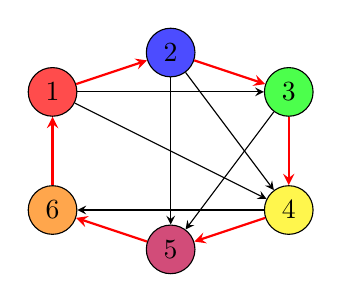
\begin{tikzpicture}[>=stealth, node distance=1.5cm]
    % Nodos con diferentes colores y posiciones más compactas
    \node[draw, circle, fill=red!70] (1) at (0,1.5) {1};
    \node[draw, circle, fill=blue!70] (2) at (1.5,2) {2};
    \node[draw, circle, fill=green!70] (3) at (3,1.5) {3};
    \node[draw, circle, fill=yellow!70] (4) at (3,0) {4};
    \node[draw, circle, fill=purple!70] (5) at (1.5,-0.5) {5};
    \node[draw, circle, fill=orange!70] (6) at (0,0) {6};

    % Aristas del ciclo hamiltoniano (en rojo con flechas)
    \draw[thick, red, ->] (1) -- (2);
    \draw[thick, red, ->] (2) -- (3);
    \draw[thick, red, ->] (3) -- (4);
    \draw[thick, red, ->] (4) -- (5);
    \draw[thick, red, ->] (5) -- (6);
    \draw[thick, red, ->] (6) -- (1);

    % Otras aristas adicionales (negras)
    \draw[->] (1) -- (3);
    \draw[->] (1) -- (4);
    \draw[->] (2) -- (4);
    \draw[->] (2) -- (5);
    \draw[->] (3) -- (5);
    \draw[->] (4) -- (6);

\end{tikzpicture}
\end{center}
\[
\text{cost} =
\begin{bmatrix}
  \infty & 1 & 1 & 1 & 1 & 1 & 1 \\
  1 & \infty & 1 & 1 & 1 & \infty & \infty \\
  1 & \infty & \infty & 1 & 1 & 1 & \infty \\
  1 & \infty & \infty & \infty & 1 & 1 & \infty \\
  1 & \infty & \infty & \infty & \infty & 1 & 1 \\
  1 & \infty & \infty & \infty & \infty & \infty & 1 \\
  1 & 1 & \infty & \infty & \infty & \infty & \infty
\end{bmatrix}

\text{pickup\_places} =
\begin{bmatrix}
  -1 & 1 & 2 & 6 & 46 & 60 & 48
\end{bmatrix}
\]

\end{center}






\textbf{Correctitud}

Existe un ciclo Hamiltoniano en \( G \) de tamaño \(\iff\) existe una ruta de costo \(n+2\) con las entradas \(cost\) y \(pickup\_places\).

\begin{itemize}
    \item \(\Leftarrow\) 
    Sea r una posible ruta de recogida y entrega de productos de costo \(n+2\), entonces \(r = [x_1,x_2,...,x_n,x_{n+1},x_{n+2},x_{n+3}]\), ya que para que el costo de una ruta sea \(m\) esta debe tener \(m+1\) lugares, pues los únicos posibles costos de viajar entre dos lugares son \(1\) y \(\infty\), y de existir \(cost[x_i][x_j]= \infty\), con \(i<j\) el costo de la ruta sería \(\infty\). Además, se cumple que \(x_1=x_{n+3}=0\), ya que la ruta debe iniciar en el almacén y terminar en este. Todos los lugares deben ser visitados al menos una vez para que se les pueda entregar los productos, y existen \(n\) lugares diferentes sin contar el origen.Como en \([x_2,...,x_{n+1},x_{n+2}]\) hay \(n+1\) lugares, entonces hay un lugar que es visitado dos veces, este lugar es \(x_2\), ya que al visitar \(x_2\) no se le puede entregar su producto, ya que este no ha sido recogido, pues el único lugar que se visitó antes fue el origen, que no contiene ningún producto. Si \(x_2 = x_i\), con \(i<n+2\), entonces \(x_{n+2} \neq x_2\), por lo que \(x_{n+2}\) solo aparece una vez, entonces el producto recogido en \(x_{n+2}\) no puede ser entregado en ningún lugar, ya que el único lugar que es visitado después, es el origen. Por tanto, se cumple que \(x_2 = x_{n+2}\). Dado \(r\), es posible obtener un ciclo \(c\) en \(G\) que contenga todos los vértices una sola vez, \(c = [x_2,...,x_n,x_{n+1},x_2]\), pues a cada par \(x_k,x_{k+1} \in r\), le corresponde un arco \((x_k,x_{k+1}) \in E\), pues en caso contrario \(cost[x_k][x_{k+1}] \neq 1\). Por tanto, por cada ruta válida con costo \(n+2\), existe un ciclo hamiltoniano en \(G\).

    \item \(\Rightarrow\) 
    Dado un ciclo hamiltoniano \(h\) en \(G\), con \(h=[x_2,x_3,...,x_n,x_{n+1},x_2]\), es posible construir una ruta válida de costo \(n+2\) para el problema de recogida y entrega de productos. Sea \(r=[0,x_2,x_3,...x_n,x_{n+1},x_2,0]\), esta ruta satisface las dependencias expresadas en \(pickup\_places\), pues  \(pickup\_places[x_{k+1}] \& 2^{x_k} \neq 0\), ya que \((x_k,x_{k+1})\in E\). Además, el costo de \(r\) es \(n+2\), pues \(cost[x_k][x_{k+1}]=1 \forall x_k \in r \) y \(cost[0][x_2]=cost[x_2][0]=1\) y contiene todos los lugares porque \(h\) es un ciclo hamiltoniano. Por tanto, se cumple que por cada ciclo hamiltoniano en \(G\), existe una ruta válida de recogida y entrega de productos con entradas \(cost\) y \(pickup\_places\).
 
    

\end{itemize}

\textbf{Extensión al problema de Optimización}

Existe conjunto de retroalimentación de arcos de tamaño mínimo en \(G\) \(\iff\) existe un conjunto de retroalimentación de arcos en \(G\) de tamaño \(k\), con \(k \geq 0\).
\begin{itemize}
    \item \(\Leftarrow\) 
    Se cumple por Principio del Buen Orden.
    \item \(\Rightarrow\) 
    Si existe un conjunto de retroalimentación de arcos de tamaño mínimo \(l\), al agregar \(k-l\) vértices al conjunto, este va a seguir cumpliendo que es un conjunto de retroalimentación de arcos.
\end{itemize}

El \textbf{Problema de Recogida y Entrega de Productos}  es una especialización del \textbf{Problema de Recogida y Entrega de Productos Extendido}, donde la matriz de costes es simétrica y el coste de viajar de un lugar a él mismo es \(0\). Además, la máscara de bits solo tiene un bit activo, por lo que \(pickup_places\) solo tiene el número del bit activo por cada lugar, en el caso del origen, \(pickup_places[0]=-1\). Por tanto, el \textbf{Problema de Recogida y Entrega de Productos} también es NP-Hard.

\subsection{Soluciones}
Dado que el \textbf{Problema de Recogida y Entrega de Productos} pertenece a la clase de problemas NP-difíciles, es decir, para los cuales no se conoce un algoritmo que los resuelva en tiempo polinomial en el peor caso, en esta sección se presenta una solución exacta para el problema formulado, así como algoritmos metaheurísticos que permiten obtener soluciones aproximadas cercanas al óptimo.
\subsubsection{Solución exacta}
El problema plateado es muy similar al \textbf{Problema del Viajante}(TSP)\cite{Applegate2006}, pues consiste en hallar la ruta de menor costo. A diferencia de TSP, el problema de Recogidas y entregas presenta restricciones que limitan el orden en que son visitados los lugares. 
Un lugar puede ser visitado con dos propósitos: recoger el producto que se encuentra en este lugar o entregar el producto solicitado. Si un lugar \(x\) es visitado para recoger su producto lo denominaremos \(x'\) y si es visitado para entregar un producto lo denominaremos \(x''\). Por tanto, la ruta que optimiza el proceso visita como máximo cada lugar dos veces, ya que en cada lugar se recoge y se entrega un único producto. El origen, a su vez, es visitado solo al principio y al final de la ruta. Por ende, la entrada de este problema puede ser modificada para ser resuelto con un algoritmo que resuelva TSP, donde no se tengan en cuenta las permutaciones inválidas . Dado que se tienen \(x_1,x_2,...,x_{n-1},x_n\) lugares. Un permutación \(p\) que representa una posible ruta de vistas a lugares para recoger y entregar productos, está formada por \(x_i'\) y \(x_i''\) \(\forall i |  1 \leq i \leq n\), ya que los productos deben ser recogidos y entregados por cada uno de los lugares. Una permutación \(p\) es inválida  si y solo si:
\begin{itemize}
    \item \(x_i''\) aparece antes que \(x_i'\).
    \item \(x_i''\) aparece antes que \(x_j'\), donde \(x_j\) es el lugar donde se recoge el producto que debe entregarse en \(x_i\), o sea, \(pickup\_places[x_i]=x_j\).
\end{itemize}

Por tanto, una ciudad solo debe visitarse si no invalida la ruta que se tiene hasta el momento.

Es creada una nueva matriz de costos \(new\_cost\), de forma tal que \(new\_cost[x_i'][x_i'']=0\), ya que visitar un lugar para entregar un producto después de que fue visitado para recoger su producto, es quivalente a visitar ese lugar una única vez. Además \(new\_cost[x_i'][x_j']=new\_cost[x_i''][x_j'']=new\_cost[x_i'][x_j'']=new\_cost[x_i''][x_j']=cost[x_i][x_j]\). Esta es la entrada al algoritmo que resuelve TSP, junto con el ciclo de deependencias, donde se añaden verificaciones para no formar permutaciones inválidas. 

\textbf{Complejidad}
La solución propuesta es una modificación de la implementación del algoritmo que resuelve el Problema del Viajante con un enfoque de programación dinámica, cuya complejidad temporal es \(\mathcal{O}(n^2*2^n)\). Las verificaciones añadidas funcionan en tiempo constante, por tanto, la complejidad temporal del algoritmo propuesto no varía, y es \(\mathcal{O}(n^2*2^n)\). 

\subsubsection{Algoritmo de Optimización por Colonias de Hormigas}

En la naturaleza, las hormigas encuentran caminos óptimos entre su nido y las fuentes de alimento depositando feromonas sobre el suelo. Cuando muchas hormigas transitan por un mismo camino, la concentración de feromonas se refuerza, haciendo que otras hormigas sean más propensas a seguir esa ruta. Con el tiempo, la ruta más corta (o de mayor eficiencia) tiende a recibir más refuerzo, ya que las hormigas que la utilizan depositan feromonas más frecuentemente debido a que la recorren en menos tiempo.

\begin{figure}[h]
    \centering
    \includegraphics[width=0.5\textwidth]{ant_rute.png}
    \caption{Rutas de las hormigas}
    \label{fig:gadget}
\end{figure}

 En esta solución, las hormigas van construyendo recorridos (posibles soluciones al problema) moviéndose por el grafo de un punto a otro hasta que completan un ciclo. Para ello, primeramente se inicializa una matriz de feronmonas con un valor pequeño y constante, como el total de  clientes. Luego en cada iteración del algoritmo, cada hormiga construye su recorrido ejecutando una regla de transición probabilista que indica qué nodo debe añadir al ciclo que está construyendo. El número de iteraciones máximo que se deja correr al algoritmo depende de la decisión del usuario, ya que no hay un mecanismo a priori que diga si alguna hormiga ya ha encontrado la solución óptima. \cite{ant}

Para cada hormiga, la transición de la ciudad \textit{i} a la ciudad \textit{j} en una iteración del algoritmo depende de:
\begin{itemize}
    \item \textbf{Si un cliente ha sido ya visitado o no, en el ciclo que está construyendo}: Cada hormiga mantiene en memoria los clientes que ya han visitado en el recorrido actual, y únicamente considera en cada paso los clientes que no han visitado todavía, que denotaremos por $J_i^k$ (clientes no visitados por la hormiga \textit{k} en esta iteración). De esta forma, aseguramos que al final la hormiga ha 
    construido un recorrido válido.
    \item \textbf{La inversa de la distancia a dicho cliente, \(\nu_{ij} = 1/d_{ij}\), que es lo que se llama visibilidad}: Esta medida informa acerca de la bondad de escoger \( C_j \) estando en \( C_i \), y puede ser usada por las hormigas para que la distancia entre los clientes consecutivos sea una característica que intervenga en la selección del recorrido que se está construyendo.
    \item \textbf{La cantidad de feromona que hay depositada en la arista que une ambos nodos, que denotaremos por \(\tau_{ij}(t)\)}: Esta cantidad se actualiza en cada paso, dependiendo de la cantidad de hormigas que han pasado por ella y de que el recorrido final de las hormigas que han usado esta conexión haya sido bueno (en relación con los demás caminos explorados). De alguna forma, mide la inteligencia colectiva del hormiguero, ya que es información que depende del conjunto de hormigas que están realizando la búsqueda.
\end{itemize}

A partir de las anteriores consideraciones, la probabilidad de que la hormiga \textit{k} vaya de \(C_i\) a \(C_j\) en la construcción del recorrido actual, viene dada por una expresión del tipo siguiente:

\[
p_{ij}^k(t) =
\begin{cases}
\frac{[\tau_{ij}(t)]^\alpha [\nu_{ij}]^\beta}{\sum\limits_{l \in J_i^k} [\tau_{il}(t)]^\alpha [\nu_{il}]^\beta}, & \text{si } j \in J_i^k \\[10pt]
0, & \text{si } j \notin J_i^k
\end{cases}
\]

Donde \(\alpha\) y \(\beta\) son dos parámetros ajustables que controlan el peso relativo de cada una de las medidas en la heurística resultante.

Con el fin de mejorar los recorridos más prometedores para el problema, y tras completar cada ciclo, cada hormiga deposita una cantidad de feromona, \(\Delta \tau_{ij}^k(t)\), en cada una de las aristas del ciclo que ha construido. Esta cantidad dependerá de lo bueno que ha sido ese recorrido en comparación con el del resto de las hormigas.

Por ejemplo, si la hormiga \textit{k} ha realizado el recorrido \(T^k(t)\), de longitud total \(L^k(t)\), para cada par \((i,j) \in T^k(t)\), se puede hacer un depósito de feromona de \(\Delta \tau_{ij}^k(t) = Q/L^k(t)\) donde \(Q\) es un parámetro del sistema (en la práctica, este parámetro se ajusta para que la influencia de ambas estrategias sea compensada). \cite{ant}


De esta forma, los recorridos más largos tendrán menos ganancia de feromona en sus aristas, lo que disminuirá su probabilidad relativa de ser seleccionados en etapas posteriores. 

\begin{figure}[h]
    \centering
    \includegraphics[width=0.5\textwidth]{pheromones_distribution.png}
    \caption{Distribución de feromonas en las rutas}
    \label{fig:gadget}
\end{figure}

Para que este método funcione correctamente es necesario, además, dejar que la feromona no permanezca indefinidamente, sino que su influencia decaiga en el tiempo. Así, aquellas aristas que no vuelvan a ser visitadas por las hormigas (y que, por tanto, no son reforzadas), tendrán cada vez menos influencia en la heurística de decisión de cada paso.

Para conseguir este efecto, en los algoritmos de hormigas se introduce un nuevo parámetro, \(0 \leq \rho \leq 1\), junto con una regla de actualización de feromona como sigue:
\[\tau_{ij}(t) \longleftarrow (1-\rho)\tau_{ij}(t) +  \Delta \tau_{ij}^k(t)\]
y se supone que, inicialmente, en todas las aristas hay una cantidad pequeña de feromona, \(\tau_0\).

El número total de hormigas que intervienen, que hemos denotado por {M} en la ecuación anterior, es otro parámetro importante a tener en cuenta:
\begin{itemize}
    \item Demasiadas hormigas tenderán rápidamente a reforzar recorridos que no son óptimos, por lo que puede ser difícil que el grupo los olvide y encontrar mejores opciones,
    \item muy pocas hormigas no provocarán el proceso de sinergia esperado, ya que no pueden contrarrestar el efecto de la evaporación de feromona, por lo que, finalmente, la solución que proporcionen sería equivalente al del algoritmo voraz estocástico \cite{ant}
\end{itemize}

La complejidad de esta solución es \(O(I·A·n^2)\) siendo \(I\) la cantidad de iteraciones, \(A\) la cantidad de hormigas y \(n\) el número de clientes (si se escoge \(A=n\) entonces la complejidad quedaría \(O(I·n^3)\)). Esta complejidad es debido a que por cada iteración del algoritmo, cada hormiga construye una ruta posible y calcula su distancia total. Realizar estas acciones serían en total \(O(n^2)\). Por tanto, la complejidad es la dicha anteriormente.

\subsubsection{Algoritmo Genético}

El Algoritmo Genético (AG) es una técnica de resolución de problemas que se inspira en la evolución biológica como estrategia para la resolución, englobándose en técnicas basadas en poblaciones. Dado un problema específico a resolver, la entrada del AG es un conjunto de soluciones potenciales a ese problema, codificadas de alguna manera, y una métrica llamada función de aptitud, o \textit{fitness}, que permite evaluar cuantitativamente la bondad de cada solución candidata. En el problema de la distribución de los medicamentos, la entrada de AG es un conjunto de rutas posibles y la función de aptitud es la longitud de cada ruta, de manera que la mejor ruta es la que minimiza la distancia total.  

A partir de ahí, AG evalúa cada candidata de acuerdo con la función de aptitud. Por supuesto, se debe tener en cuenta que estas primeras candidatas mostrarán baja eficiencia con respecto a la resolución del problema, y la mayoría no funcionarán en absoluto. Sin embargo, por puro azar, unas pocas pueden ser prometedoras, pudiendo mostrar algunas características que muestren, aunque solo sea de una forma débil e imperfecta, cierta capacidad de solución del problema. Estas candidatas prometedoras son escogidas por un proceso de selección. Entre las técnicas de selección se encuentran los torneos, que eligen subgrupos de individuos de la población, y los miembros de cada subgrupo compiten entre ellos. Sólo se elige a un individuo de cada subgrupo para la reproducción.  

Estas candidatas prometedoras se conservan y se les permite reproducirse. Las características individuales de las candidatas se combinan por medio de operaciones de cruzamiento para generar nuevos descendientes (simulando lo que sería la reproducción sexual). En el problema en cuestión se utiliza el \textit{Order Crossover - OX}, que a diferencia del cruzamiento de un punto, dos puntos y el uniforme, en este cruzamiento se respeta el principio de permutación y cada elemento aparece en un individuo una sola vez.

\begin{figure}[h]
    \centering
    \includegraphics[width=0.5\textwidth]{Diagram-of-ordered-crossover.jpg}
    \caption{Diagrama del \textit{Order Crossover}.}
    \label{fig:gadget}
\end{figure}

Luego, se generan múltiples copias de ellas, pero estas copias no son perfectas, ya que durante el proceso de duplicación se introducen algunos cambios aleatorios, similares a las mutaciones que pueden sufrir los descendientes de una población. Esta descendencia digital continúa en la siguiente generación, formando un nuevo conjunto de soluciones candidatas, las cuales son nuevamente sometidas a una ronda de evaluación de aptitud. Las candidatas que han empeorado o no han mejorado con las mutaciones son eliminadas; sin embargo, por puro azar, las variaciones aleatorias introducidas en la población pueden haber mejorado a algunos individuos, convirtiéndolos en soluciones del problema más completas o eficientes. El proceso se repite las iteraciones que sean necesarias hasta que se obtengan soluciones suficientemente buenas.

Podemos dar una primera formalización del proceso anterior por medio del siguiente pseudocódigo: 

\begin{figure}[h]
    \centering
    \includegraphics[width=0.5\textwidth]{pseuddocodigo_genetic.png}
    \label{fig:gadget}
\end{figure}

Aunque pueda parecer asombroso, anti-intuitivo, y quizás como algo de suerte y magia, los AG han demostrado ser una estrategia enormemente poderosa y exitosa para resolver problemas, mostrando de manera espectacular el poder de los principios evolutivos. Además, las soluciones que consiguen son a menudo más eficientes, más elegantes o más complejas que las que un humano produciría. 

Este algoritmo de aproximación posee una complejidad \(O(G \cdot P \cdot n²)\), siendo \(G\) la cantidad de generaciones o iteraciones del algoritmo, \(P\) el tamaño de la población y \(n\) la cantidad de clientes. Se puede comprobar, pues:
\begin{itemize}
    \item Crear la población: Se generan P rutas, cada una con complejidad O(n) $\rightarrow$ \(O(P \cdot n)\)
    \item Por cada generación se escoge la mitad de la población y por cada individuo se realizan dos veces la selección, cruzamiento y mutación. La selección se realiza en \(O(n)\), el cruzamiento en \(O(n^2)\) y la mutación en \(O(1)\). Antes de terminar la iteración, se calculan las distancias de cada uno de los individuos de la población y se ordenan, en \(O(n\cdot P \cdot \log P )\). 
    \item Por tanto, la complejidad total, sería \(O(P \cdot n + G \cdot n\cdot P \cdot \log P + G \cdot P \cdot n^2) = O(G \cdot P \cdot n^2)\). 
\end{itemize}

\rule{\linewidth}{0.5pt}

\section{Conclusiones}

\renewcommand\refname{Referencias}

\begin{thebibliography}{}

  \sloppypar
  \bibitem{ant} Sancho Caparrini, Fernando (2018). Hormigas y el Problema del Viajante. Noviembre, 2018.  
  \bibitem{Applegate2006} Applegate, D. L., Bixby, R. E., Chvátal, V.,  Cook, W. J. (2006). The Traveling Salesman Problem: A Computational Study. Princeton University Press.  
\end{thebibliography}

\end{document}